\documentclass{beamer}

\usepackage{amsfonts}
\usepackage{amsmath}
\usepackage{longtable}
\usepackage{csquotes}
\usepackage{standalone}

\usepackage{graphicx}
\graphicspath{{../pictures/}}

\usepackage{tikz}
\usetikzlibrary{shapes, calc, arrows, decorations.markings,
  decorations.pathmorphing, decorations, patterns, chains, snakes,
  backgrounds, positioning, fit, petri}
\newcommand{\inputpicture}[1]{\input{../drawings/#1}}

\usepackage{listings}
\lstset{language=C, basicstyle=\ttfamily, breaklines=true, keepspaces=true,
  keywordstyle=\color{blue}}

\usepackage{bytefield}

\usefonttheme{professionalfonts}
\usefonttheme{serif}
\usepackage{fontspec}
\setromanfont{CMU Serif}
\setsansfont{CMU Sans Serif}
\setmonofont{CMU Typewriter Text}

\usepackage{hyperref}
\hypersetup{colorlinks=true, linkcolor=black, filecolor=black, citecolor=black,
  urlcolor=blue , pdfauthor=Evgenii Iuliugin <yulyugin@gmail.com>,
  pdftitle=Fundamentals of Full-Platform Simulation}

\usepackage{underscore}
\usepackage{amsthm}

\subtitle{Fundamentals of Full-Platform Simulation}
\subject{Lecture}
\date{\today}

\author[Evgenii Iuliugin]{
  Evgenii Iuliugin \small{\href{mailto:yulyugin@gmail.com}{yulyugin@gmail.com}}}
\typeout{Copyright 2021 Evgenii Iuliugin}

\usetheme{Berlin}
\setbeamertemplate{navigation symbols}{}

\newcommand{\finalslide}{
    {\huge{Thank you!}\par}

    \vfill
    Slides and material are available at
    \url{https://github.com/yulyugin/sim-lectures}
    \vfill

    \tiny{\textit{Note}: All trademarks are the property of their respective
        owners.
        The presented point of view reflects the personal opinion of the author.

        %All the materials are licensed under the Creative Commons
        %Attribution-NonCommercial-ShareAlike 4.0 Worldwide. To view a copy of
        %this license, visit
        %\url{http://creativecommons.org/licenses/by-nc-sa/4.0/}.
    }
}


\usepackage{tikz}
\usetikzlibrary{shapes, calc, arrows, decorations.markings, decorations.pathreplacing, decorations.pathmorphing, decorations, patterns, chains, snakes, backgrounds, positioning, fit, shadows}

\title{Simulation Through Just in Time Compilation}

\begin{document}

\startslides

\begin{frame}{On the Previous Lecture:}
\begin{itemize}
\item 5-stage pipeline: \textbf{F}, \textbf{D}, \textbf{Ex}, \textbf{Mem},
  \textbf{WB}.
\item Interpreters are slow.
\item Discussed couple of improved interpreter implementations.
\end{itemize}
\end{frame}

\begin{frame}{Questions}
\begin{itemize}
\item What is a difference between decoding and disassembling?\pause
\item What is a difference between interrupt and exception?\pause
\item Can a threaded interpreter be cached as well?
\end{itemize}
\end{frame}

\begin{frame}{Simulated System}
\centering
\vfill
\inputpicture{cpu-mem}
\vfill
\end{frame}

\begin{frame}{What Was Optimized in Interpreter}
\begin{itemize}
\item \textbf<1>{Fetch} \only<1>{$\leftarrow$ optimized}
\item \textbf<1>{Decode} \only<1>{$\leftarrow$ optimized}
\item \textbf<2>{Execute} \only<2>{$\rightarrow$ to be optimized}
\item \textbf<2>{Memory} \only<2>{$\rightarrow$ to be optimized}
\item \textbf<2>{Write-Back} \only<2>{$\rightarrow$ to be optimized}
\end{itemize}
\end{frame}

\section{Interpretation, Compilation, Translation}

\begin{frame}{Translation, Compilation, Decompilation}
\pause
\begin{itemize}
\item \textbf{Translation} --- \textit{generic term} describing a process of
  code conversion from one programming language into another.
\item \textbf{Compilation} --- \textit{translation} from high-level programming
  language into low-level programming language.
\item \textbf{Decompilation} --- \textit{translation} from low-level programming
  language into a high-level programming language.
\end{itemize}
\end{frame}

\begin{frame}{Interpretation and Compilation For High-Level Programming Languages}
\begin{itemize}
\item BASIC, Python, Shell\dots
  \begin{itemize}
  \item Read a line --- detect a command --- execute the command.
  \item Slow but more <<interractive>>.
  \end{itemize}
\item Fortran, C, Pascal\dots
  \begin{itemize}
  \item First stage: read a line --- detect a command --- translate to machine code.
  \item Second stage: execute the machine code.
  \end{itemize}
\end{itemize}
\end{frame}

\begin{frame}{Binary Translation}
\begin{itemize}
\item Input: guest machine code.
\item Output: host machine code.
\item \textbf{Binary translation, BT} --- translation of guest software written in
  guest ISA into equivalent code in host ISA.
\item What for? \pause Repetitive execution of translation result. Optimizations.
\end{itemize}
\end{frame}

\begin{frame}{Static and Dynamic Binary Translation}
\begin{itemize}
\item \textit{Static} binary translator converts a target executable file
  without running it.
\item Result of static BT is saved on disk.
\item It is very difficult to do correctly.
\vfill
\item \textit{Dynamic} binary translation happens during simulation.
\item Result of dynamic BT is saved in memory.
\item Dynamic BT can adopt to program's run-time environment.
\item Dynamic BT alternates with execution of the generated code.
\end{itemize}
\end{frame}

\begin{frame}{Stages of Dynamic Binary Translation}
\centering
\inputpicture{dynamic-bt}
\end{frame}

\section{Template-Based Translation}

\begin{frame}{Algorithm 1: Template-Based Translation}
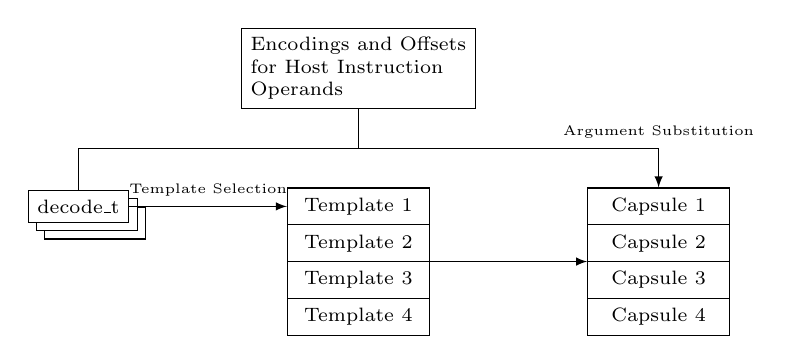
\begin{tikzpicture}[font=\scriptsize, >=latex, node distance=2.cm]

\node[draw, double copy shadow={shadow xshift=3pt,shadow yshift=-3pt}, fill=white] (decode) {decode_t};
\node[rectangle split, rectangle split parts=4, draw, right=of decode, anchor=text west, minimum width=1.8cm] (templates-raw) {Template 1\nodepart{two} Template 2\nodepart{three} Template 3\nodepart{four} Template 4};

\node[rectangle split, rectangle split parts=4, draw, right=of templates-raw, minimum width=1.8cm] (templates) {Capsule 1\nodepart{two} Capsule 2\nodepart{three} Capsule 3\nodepart{four} Capsule 4};

\node[draw, above=1cm of templates-raw, align=left] (md) {Encodings and Offsets\\for Host Instruction\\Operands};

\draw[->] (decode) -- (templates-raw.text west) node[midway, above]{\tiny Template Selection};
\draw[->] (templates-raw) -- (templates);
\coordinate[above=0.5cm of templates] (junction);
\draw[->] (decode) |- (junction) -- (templates) node[pos=0, above]{\tiny Argument Substitution};
\draw[] (md) |- (junction);
\end{tikzpicture}
\end{frame}

\begin{frame}[fragile]{Algorithm 1: Template-Based Translation}
\begin{tiny}
\begin{itemize}
    \item start_addr --- guest code's start address,
    \item start_buf --- host buffer.
\end{itemize}
\end{tiny}

\begin{lstlisting}
translate(start_addr, start_buf) {
    PC = start_addr; bufptr = start_buf;
    while (!enough) {
        instr = fetch(PC);
        (opcode, operands) = decode(instr);
        (template, length) = templates[opcode];
        memcpy(bufptr, template, length);
        patch_operands(bufptr, operands);
        PC += instr_length;
        bufptr += length;
    }
    memcpy(bufptr, glue_capsule, glue_length);
}
\end{lstlisting}
\end{frame}

\begin{frame}[fragile]{Algorithm 1: Execution}

\begin{lstlisting}
execute(start_buf) {
    load_simulated_state();
    goto start_buf;
}
\end{lstlisting}
\pause
or
\begin{lstlisting}
typedef void (*fblock)(void);
execute(start_buf) {
    load_simulated_state();
    ((fblock)start_buf)();
}
\end{lstlisting}
\end{frame}

\begin{frame}{Capsule}
\begin{small}
\begin{tabular}{p{0.45\textwidth}p{0.45\textwidth}}
Guest code, Intel~64 (64-bit) & Host code, Intel~IA-32 (32-bit)
\end{tabular}
\end{small}
\vfill
\centering
\inputpicture{capsule}
\pause
Question: What part of \texttt{ADDQ} semantics is missing?
\end{frame}

\begin{frame}{Argument Substitution}

{\ttfamily\small
{\sffamily Registers:}

\begin{tabular}{ll}  
c5 f4 58 c\textcolor{red}{8}  &    vaddps \textcolor{red}{\%ymm0},\%ymm1,\%ymm1 \\
c5 f4 58 c\textcolor{red}{9}  &    vaddps \textcolor{red}{\%ymm1},\%ymm1,\%ymm1 \\
c5 f4 58 c\textcolor{red}{f}  &    vaddps \textcolor{red}{\%ymm7},\%ymm1,\%ymm1 \\\pause
c4 c1 74 58 c\textcolor{red}{8} &  vaddps \textcolor{red}{\%ymm8},\%ymm1,\%ymm1 \\
c4 c1 74 58 c\textcolor{red}{f} &  vaddps \textcolor{red}{\%ymm15},\%ymm1,\%ymm1 \\
c5 f4 58 c8  &    vaddps \%ymm0,\%ymm1,\%ymm1 \\
c5 ec 58 d0  &    vaddps \%ymm0,\%ymm2,\%ymm2 \\
c5 c4 58 f8  &    vaddps \%ymm0,\%ymm3,\%ymm3 \\\pause
c4 e1 74 58 c8 &  vaddps \%ymm0,\%ymm1,\%ymm1 \# Mnemonic is the same!\\
\end{tabular}
\pause
{\sffamily Literals:}
\begin{tabular}{ll}
67 c7 85 \textcolor{blue}{00 01 00 00} \textcolor{green}{dd cc bb aa}   & movl \textcolor{green}{\$0xaabbccdd},\textcolor{blue}{0x100}(\%ebp)
\end{tabular}
}

\end{frame}

\section{Translation with Intermediate Representation}

\begin{frame}{Algorithm 2: JIT. IR generation}
\centering
\begin{tikzpicture}[font=\small, >=latex]

\node[rectangle split, rectangle split parts=2, draw, double copy shadow={shadow xshift=3pt,shadow yshift=-3pt}, fill=white] (sr) {Simulation routine\nodepart{two} С (subset)};
\node[rectangle split, rectangle split parts=2, draw, below=1cm of sr, double copy shadow={shadow xshift=3pt,shadow yshift=-3pt}, fill=white] (template) {Template\nodepart{two} IR: bytecode+SSA};
\draw[->] (sr) -- (template) node[midway, right] {SR-compiler};

\end{tikzpicture}
\end{frame}

\begin{frame}{Algorithm 2: JIT. Simulation Stage}
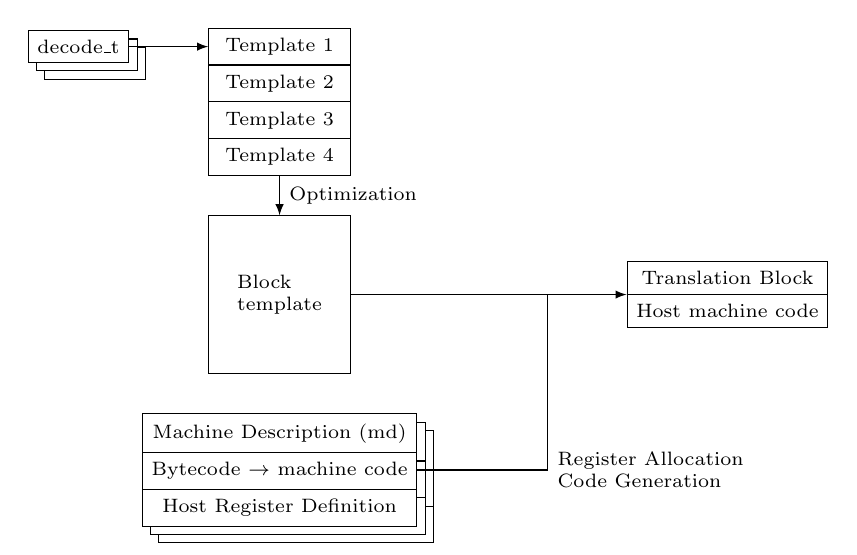
\begin{tikzpicture}[font=\scriptsize, >=latex, node distance=1.cm]

\node[draw, double copy shadow={shadow xshift=3pt,shadow yshift=-3pt}, fill=white] (decode) {decode_t};
\node[rectangle split, rectangle split parts=4, draw, right=of decode, anchor=text west, minimum width=1.8cm] (templates) {Template 1\nodepart{two} Template 2\nodepart{three} Template 3\nodepart{four} Template 4};
\draw[->] (decode) -- (templates.text west);

\node[draw, below=0.5cm of templates, minimum height=2cm, align=left, minimum width=1.8cm] (opt-template) {Block\\template};
\draw[->] (templates) -- (opt-template) node[midway, right] {Optimization};

\node[rectangle split, rectangle split parts=3, align=left, draw, below=0.5cm of opt-template, double copy shadow={shadow xshift=3pt,shadow yshift=-3pt}, fill=white] (md) {Machine Description (md)\nodepart{two} Bytecode $\rightarrow$ machine code\nodepart{three} Host Register Definition};

\coordinate[right=2.5cm of opt-template] (junction);

\node[draw, right=1cm of junction, rectangle split, rectangle split parts=2,] (host-code) {Translation Block\nodepart{two} Host machine code};

\draw[->] (md) -| node[pos=0.5, right, align=left] {Register Allocation\\Code Generation} (junction) -- (host-code);
\draw[] (opt-template) -- (junction);

\end{tikzpicture}
\end{frame}

\begin{frame}{Optimizations}
\centering
\inputpicture{bt-optimization}
\end{frame}

\begin{frame}{Connection between Translation Blocks}
\centering
\inputpicture{bb-translation}
\end{frame}

\begin{frame}{Why Optimizations During BT Are Complicated?}

\begin{itemize}
\item Machine code has less information about the algorithm compared to code in
  high-level programming languages.
\item Many compiler optimizations cannot be used.
\item BT optimizations are limited in time.
\end{itemize}
\pause
\begin{itemize}
\item Variable addresses --- not available.
\item Function boundaries --- not available.
\item Branch addresses --- partially known.
\end{itemize}
\end{frame}

\section{Difficulties of Binary Translation}

\begin{frame}{Self Modifying Code}
\centering
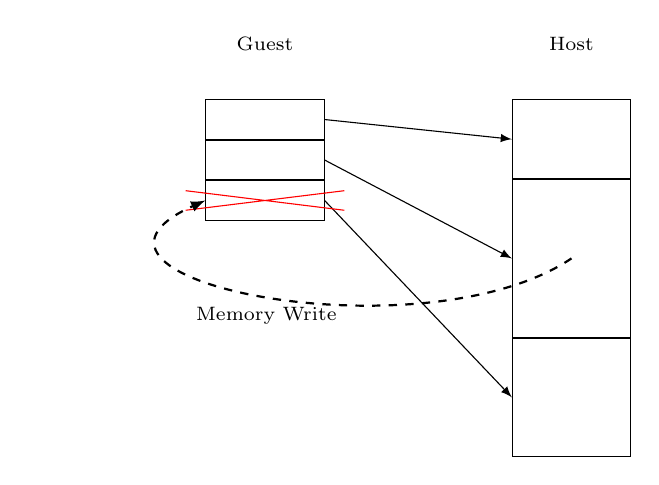
\begin{tikzpicture}[font=\scriptsize, >=latex]
    \node (guest) {Guest};
    \node[right=3cm of guest] (host) {Host};

    \node[draw, minimum width = 1.5cm, minimum height = 0.5cm, below =0.5cm of guest] (gi1) {};
    \node[draw, minimum width = 1.5cm, minimum height = 0.5cm, below = 0cm of gi1] (gi2) {};
    \node[draw, minimum width = 1.5cm, minimum height = 0.5cm, below = 0cm of gi2] (gi3) {};

    \node[draw, minimum width = 1.5cm, minimum height = 1cm, below =0.5cm of host] (hi1) {};
    \node[draw, minimum width = 1.5cm, minimum height = 2cm, below = 0cm of hi1] (hi2) {};
    \node[draw, minimum width = 1.5cm, minimum height = 1.5cm, below = 0cm of hi2] (hi3) {};

    \draw[->] (gi1.east) to (hi1.west);
    \draw[->] (gi2.east) to (hi2.west);
    \draw[->] (gi3.east) to (hi3.west);
    \pause
    \node[draw = red, minimum width = 2cm, cross out] at (gi3) {};
    \draw[->, dashed, thick, ] (hi2.center) .. controls (2, -4) and (-3, -3) .. (gi3.west) node[pos=0.5, below] {Memory Write};
\end{tikzpicture}
\end{frame}

\begin{frame}{Code Detection 1}
\begin{itemize}
    \item Find instruction boundaries,
    \item Distinguish code from data.
\end{itemize}
\centering
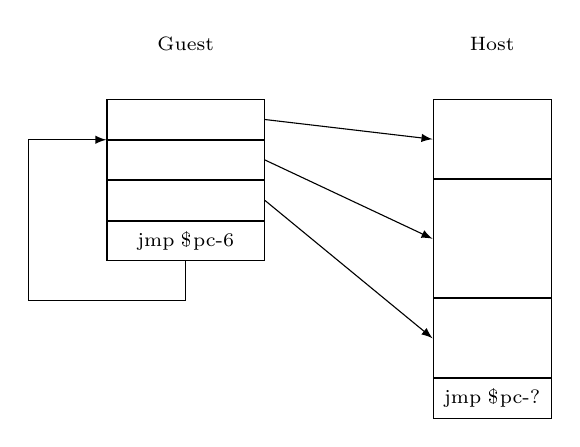
\begin{tikzpicture}[font=\scriptsize, >=latex]
    \node (guest) {Guest};
    \node[right=3cm of guest] (host) {Host};

    \node[draw, minimum width = 2cm, minimum height = 0.5cm, below =0.5cm of guest] (gi1) {};
    \node[draw, minimum width = 2cm, minimum height = 0.5cm, below = 0cm of gi1] (gi2) {};
    \node[draw, minimum width = 2cm, minimum height = 0.5cm, below = 0cm of gi2] (gi3) {};
    \node[draw, minimum width = 2cm, minimum height = 0.5cm, below = 0cm of gi3] (gjmp) {jmp \$pc-6};

    \node[draw, minimum width = 1.5cm, minimum height = 1cm, below =0.5cm of host] (hi1) {};
    \node[draw, minimum width = 1.5cm, minimum height = 1.5cm, below = 0cm of hi1] (hi2) {};
    \node[draw, minimum width = 1.5cm, minimum height = 1cm, below = 0cm of hi2] (hi3) {};
    \node[draw, minimum width = 1.5cm, minimum height = 0.5cm, below = 0cm of hi3] (hi4) {jmp \$pc-?};

    \draw[->] (gi1.east) to (hi1.west);
    \draw[->] (gi2.east) to (hi2.west);
    \draw[->] (gi3.east) to (hi3.west);

    \draw[->] (gjmp.south) |- ([xshift=-2cm, yshift=-0.5cm]gjmp.south) |- (gi1.south west);
    
\end{tikzpicture}

\end{frame}

\begin{frame}{Code Detection 2}
\begin{center}
\inputpicture{byte-shift}
\end{center}

That's why static BT is not always possible.
\end{frame}

\begin{frame}{Outrunning Translation}
\centering
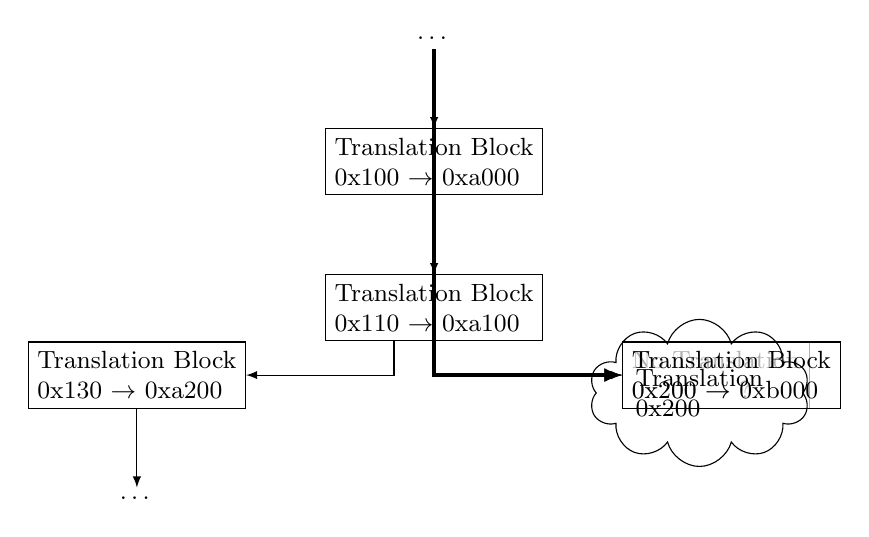
\begin{tikzpicture}[>=latex, font=\small, align=left]
    \node[draw] (tb100) {Translation Block\\0x100 $\rightarrow$ 0xa000};
    \node[above=of tb100] (pred) {\dots};
    \node[draw, below= of tb100] (tb110) {Translation Block\\0x110 $\rightarrow$ 0xa100};
    \node[draw, left=of tb110.south west, anchor=north east] (tb130) {Translation Block\\0x130 $\rightarrow$ 0xa200};
    \node[below=of tb130] (cont) {\dots};
    \draw[->] (tb100) -- (tb110);
    \draw[->] (tb110.220) |- (tb130);
    \draw[->] (tb130) -- (cont);
    \draw[->] (pred) -- (tb100);
    
    \uncover<1-2>{\node[draw=black!30, right=of tb110.south east, anchor=north west, text=black!30] (notb200) {No Translation\\0x200 $\rightarrow$ ?};}
    \uncover<2>{\draw[->, very thick] (pred) -- (tb100.center) -- (tb110.center) |- (notb200);}

    \uncover<3>{\node[draw, right=of tb110.south east, anchor=north west, cloud, aspect=2]  (in-progress) {Translation\\0x200};}

    \uncover<4->{\node[draw, right=of tb110.south east, anchor=north west] (tb200) {Translation Block\\0x200 $\rightarrow$ 0xb000};}
    \uncover<4->{\draw[->] (tb110) |- (tb200);}

    \uncover<5>{\draw[->, very thick] (pred) -- (tb100.center) -- (tb110.center) |- (tb200);}
\end{tikzpicture}
\end{frame}

\begin{frame}{Hot Path Translation}
\only<1>{Execution 1: use interpreter with tracing.}
\only<2>{Execution $N$: detect a <<hot path>> in the trace.}
\only<3>{Translate the <<hot path>> into a block.}
\only<4>{Insert the new block into the trace.}
\vfill
\centering
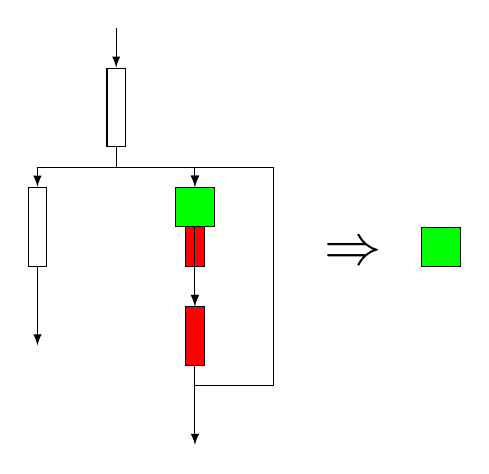
\begin{tikzpicture}[>=latex, font=\small]
\uncover<1,2,4>{
    \coordinate (pred);
    \node[draw, below=0.5cm of pred, minimum height=1cm] (tb1) {};
    \coordinate[below=0.25cm of tb1] (jp1);
    \coordinate[below=0.25cm of jp1] (jp2);
    \node[draw, minimum height=1cm, left=of jp2, anchor=north] (tb2) {};
}
\uncover<1-3>{
    \node[draw, minimum height=1cm, right=of jp2, anchor=north] (tb3) {};
    \node[draw, minimum height=0.75cm, below=0.5cm of tb3] (tb4) {};
}
\uncover<2>{\node[draw, fill=red, minimum height=1cm, right=of jp2, anchor=north] (tb3-hot) {};}
\uncover<2>{\node[draw, fill=red, minimum height=0.75cm, below=0.5cm of tb3] (tb4-hot) {};}

    \coordinate[below=of tb2] (post2);
    \coordinate[below=of tb4] (post4);
\uncover<1,2>{\draw[->] (tb4) -- (post4);}
\uncover<1,2,4>{
    \draw[->] (pred) -- (tb1);
    \draw[->] (tb1.south) -- (jp1) -| (tb2);
    \draw[->] (tb1.south) -- (jp1) -| (tb3);
    \draw[->] (tb2) -- (post2);
}
\uncover<1,2,3>{
    \draw[->] (tb3) -- (tb4);
    \draw[->] (tb4.south) -- ([yshift=-0.25cm]tb4.south) -| ([xshift=1cm, yshift=0.25cm]tb3.north) -| (tb3);
}

\uncover<3>{
    \node[draw, fill=green, minimum height=0.5cm, minimum width=0.5cm, right=3cm of tb3, anchor=north] (tb5-temp) {};
    \path (tb3.south) -- (tb5-temp) node[pos=0.7] {\huge $\Rightarrow$};   
}

\uncover<4>{
    \node[draw, fill=green, minimum height=0.5cm, minimum width=0.5cm, right=of jp2, anchor=north] (tb5) {};
    \draw[->] (tb5) -- (tb4);
}    
\end{tikzpicture}
\end{frame}

\section{Conclusions}

\begin{frame}{Summary}
\begin{itemize}
\item Interpretation, Compilation, Translation.
\item Binary Translation.
\item Static and Dynamic Binary Translation.
\item Template, Capsule.
\item Intermediate Representation.
\item Self-Modifying Code.
\item Code Detection.
\item Optimization Complexities in Binary Translation.
\end{itemize}
\end{frame}

\begin{frame}[allowframebreaks]{Bibliography}
\begin{thebibliography}{99}
  \bibitem{} \textit{Jim Smith and Ravi Nair}. Virtual Machines: Versatile
  Platforms for Systems and Processes.
  \bibitem{} \textit{Fabrice Bellard}. QEMU, a Fast and Portable Dynamic
  Translator.
  \bibitem{} \textit{Anton Chernoff and Ray Hookway.} {DIGITAL FX!32} Running
  32-Bit x86 Applications on {Alpha} {NT}.
  \bibitem{} \textit{Leonid Baraz [et al.]} IA-32 Execution Layer: a Two-Phase
  Dynamic Translator Designed to Support IA-32 Applications on
  Itanium\reg-Based Systems.
\end{thebibliography}
\end{frame}

\begin{frame}{On the Next Lecture:}
\begin{itemize}
\item Direct Execution.
\item Preliminary Scanning.
\item Hardware Support.
\item{<<Gear Shifting>> for Simulation Modes.}
\end{itemize}
\end{frame}

\finalslide

\end{document}
